\pagebreak
\section{Shock Tube}
A shock tube consists of two chambers containing air ($\gamma = 1.4$) at different states, as shown below. The domain length is $L= 1$, and the diaphragm is in the middle, at $x= 0.5$.

\begin{figure}[h]
    \centering
    

\tikzset{every picture/.style={line width=0.75pt}} %set default line width to 0.75pt        

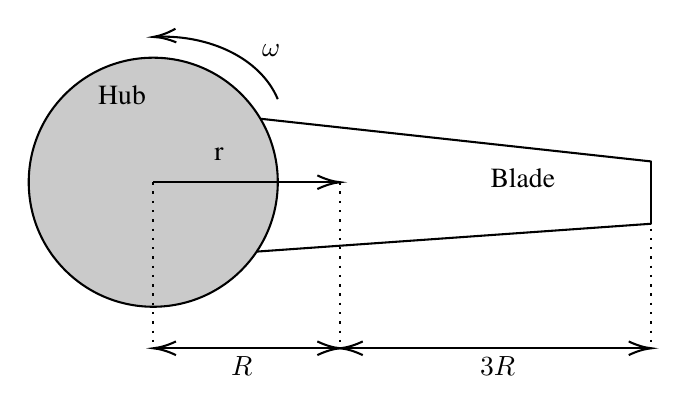
\begin{tikzpicture}[x=0.75pt,y=0.75pt,yscale=-1,xscale=1]
%uncomment if require: \path (0,300); %set diagram left start at 0, and has height of 300

%Shape: Circle [id:dp6244430308199536] 
\draw  [fill={rgb, 255:red, 202; green, 202; blue, 202 }  ,fill opacity=1 ] (220,120) .. controls (220,86.86) and (246.86,60) .. (280,60) .. controls (313.14,60) and (340,86.86) .. (340,120) .. controls (340,153.14) and (313.14,180) .. (280,180) .. controls (246.86,180) and (220,153.14) .. (220,120) -- cycle ;
%Straight Lines [id:da1433381310737285] 
\draw    (520,110) -- (520,140) ;
%Straight Lines [id:da6958270078143212] 
\draw    (520,110) -- (331.79,89.43) ;
%Straight Lines [id:da5982890152434965] 
\draw    (520,140) -- (329.79,153.43) ;
%Straight Lines [id:da7103183675633375] 
\draw    (280,120) -- (368,120) ;
\draw [shift={(370,120)}, rotate = 180] [color={rgb, 255:red, 0; green, 0; blue, 0 }  ][line width=0.75]    (10.93,-3.29) .. controls (6.95,-1.4) and (3.31,-0.3) .. (0,0) .. controls (3.31,0.3) and (6.95,1.4) .. (10.93,3.29)   ;
%Straight Lines [id:da18697245418380692] 
\draw  [dash pattern={on 0.84pt off 2.51pt}]  (280,120) -- (280,200) ;
%Straight Lines [id:da9445115873305969] 
\draw  [dash pattern={on 0.84pt off 2.51pt}]  (370,120) -- (370,200) ;
%Straight Lines [id:da8681269156370801] 
\draw    (282,200) -- (368,200) ;
\draw [shift={(370,200)}, rotate = 180] [color={rgb, 255:red, 0; green, 0; blue, 0 }  ][line width=0.75]    (10.93,-3.29) .. controls (6.95,-1.4) and (3.31,-0.3) .. (0,0) .. controls (3.31,0.3) and (6.95,1.4) .. (10.93,3.29)   ;
\draw [shift={(280,200)}, rotate = 0] [color={rgb, 255:red, 0; green, 0; blue, 0 }  ][line width=0.75]    (10.93,-3.29) .. controls (6.95,-1.4) and (3.31,-0.3) .. (0,0) .. controls (3.31,0.3) and (6.95,1.4) .. (10.93,3.29)   ;
%Straight Lines [id:da9459156094037822] 
\draw    (372,200) -- (518,200) ;
\draw [shift={(520,200)}, rotate = 180] [color={rgb, 255:red, 0; green, 0; blue, 0 }  ][line width=0.75]    (10.93,-3.29) .. controls (6.95,-1.4) and (3.31,-0.3) .. (0,0) .. controls (3.31,0.3) and (6.95,1.4) .. (10.93,3.29)   ;
\draw [shift={(370,200)}, rotate = 0] [color={rgb, 255:red, 0; green, 0; blue, 0 }  ][line width=0.75]    (10.93,-3.29) .. controls (6.95,-1.4) and (3.31,-0.3) .. (0,0) .. controls (3.31,0.3) and (6.95,1.4) .. (10.93,3.29)   ;
%Straight Lines [id:da5900923017563646] 
\draw  [dash pattern={on 0.84pt off 2.51pt}]  (520,120) -- (520,200) ;
%Curve Lines [id:da19047210809641868] 
\draw    (340,80) .. controls (331.57,59.94) and (306.65,48.98) .. (281.9,49.91) ;
\draw [shift={(280,50)}, rotate = 356.45] [color={rgb, 255:red, 0; green, 0; blue, 0 }  ][line width=0.75]    (10.93,-3.29) .. controls (6.95,-1.4) and (3.31,-0.3) .. (0,0) .. controls (3.31,0.3) and (6.95,1.4) .. (10.93,3.29)   ;

% Text Node
\draw (331,52.4) node [anchor=north west][inner sep=0.75pt]    {$\omega $};
% Text Node
\draw (316,202.4) node [anchor=north west][inner sep=0.75pt]    {$R$};
% Text Node
\draw (436,202.4) node [anchor=north west][inner sep=0.75pt]    {$3R$};
% Text Node
\draw (252,72) node [anchor=north west][inner sep=0.75pt]   [align=left] {{\fontfamily{ptm}\selectfont Hub}};
% Text Node
\draw (441,112) node [anchor=north west][inner sep=0.75pt]   [align=left] {{\fontfamily{ptm}\selectfont Blade}};
% Text Node
\draw (308,102) node [anchor=north west][inner sep=0.75pt]   [align=left] {{\fontfamily{ptm}\selectfont r}};


\end{tikzpicture}

    \caption{Shock tube chamber configuration.}
\end{figure}

At $t= 0$, the diaphragm between the two chambers is broken, sending a shock wave and a contact wave into one chamber and an expansion into the other, as shown schematically below for the density.

\begin{figure}[h]
    \centering
    

\tikzset{every picture/.style={line width=0.75pt}} %set default line width to 0.75pt        

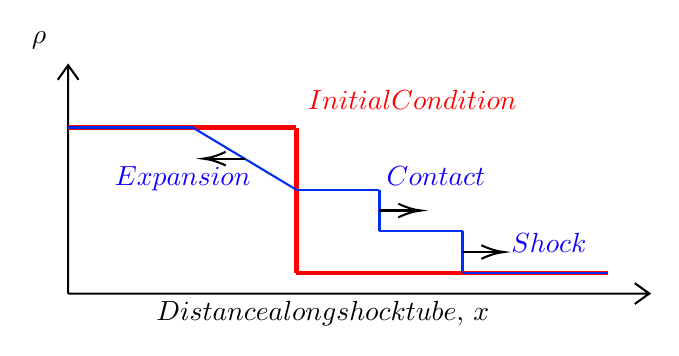
\begin{tikzpicture}[x=0.75pt,y=0.75pt,yscale=-1,xscale=1]
%uncomment if require: \path (0,300); %set diagram left start at 0, and has height of 300

%Shape: Axis 2D [id:dp2275403590324392] 
\draw  (180,170) -- (460,170)(180,60) -- (180,170) -- cycle (453,165) -- (460,170) -- (453,175) (175,67) -- (180,60) -- (185,67)  ;
%Straight Lines [id:da3604109815505028] 
\draw [color={rgb, 255:red, 255; green, 0; blue, 0 }  ,draw opacity=1 ][line width=1.5]    (180,90) -- (290,90) ;
%Straight Lines [id:da7925256894106991] 
\draw [color={rgb, 255:red, 255; green, 0; blue, 0 }  ,draw opacity=1 ][line width=1.5]    (290,90) -- (290,160) ;
%Straight Lines [id:da511794290422414] 
\draw [color={rgb, 255:red, 255; green, 0; blue, 0 }  ,draw opacity=1 ][line width=1.5]    (290,160) -- (440,160) ;
%Straight Lines [id:da6328483411928432] 
\draw [color={rgb, 255:red, 0; green, 45; blue, 235 }  ,draw opacity=1 ][line width=0.75]    (180,90) -- (240,90) ;
%Straight Lines [id:da40233058047883086] 
\draw [color={rgb, 255:red, 0; green, 45; blue, 235 }  ,draw opacity=1 ][line width=0.75]    (240,90) -- (290,120) ;
%Straight Lines [id:da7801443444674079] 
\draw [color={rgb, 255:red, 0; green, 45; blue, 235 }  ,draw opacity=1 ][line width=0.75]    (290,120) -- (330,120) ;
%Straight Lines [id:da8214841243028934] 
\draw [color={rgb, 255:red, 0; green, 45; blue, 235 }  ,draw opacity=1 ][line width=0.75]    (330,120) -- (330,140) ;
%Straight Lines [id:da6097118362505765] 
\draw [color={rgb, 255:red, 0; green, 45; blue, 235 }  ,draw opacity=1 ][line width=0.75]    (330,140) -- (370,140) ;
%Straight Lines [id:da5501138326957089] 
\draw [color={rgb, 255:red, 0; green, 45; blue, 235 }  ,draw opacity=1 ][line width=0.75]    (370,140) -- (370,160) ;
%Straight Lines [id:da6904401388837584] 
\draw [color={rgb, 255:red, 0; green, 45; blue, 235 }  ,draw opacity=1 ][line width=0.75]    (370,160) -- (440,160) ;
%Straight Lines [id:da1151620138400622] 
\draw    (265,105) -- (247,105) ;
\draw [shift={(245,105)}, rotate = 360] [color={rgb, 255:red, 0; green, 0; blue, 0 }  ][line width=0.75]    (10.93,-3.29) .. controls (6.95,-1.4) and (3.31,-0.3) .. (0,0) .. controls (3.31,0.3) and (6.95,1.4) .. (10.93,3.29)   ;
%Straight Lines [id:da9973625727389335] 
\draw    (330,130) -- (348,130) ;
\draw [shift={(350,130)}, rotate = 180] [color={rgb, 255:red, 0; green, 0; blue, 0 }  ][line width=0.75]    (10.93,-3.29) .. controls (6.95,-1.4) and (3.31,-0.3) .. (0,0) .. controls (3.31,0.3) and (6.95,1.4) .. (10.93,3.29)   ;
%Straight Lines [id:da03222983463189566] 
\draw    (370,150) -- (388,150) ;
\draw [shift={(390,150)}, rotate = 180] [color={rgb, 255:red, 0; green, 0; blue, 0 }  ][line width=0.75]    (10.93,-3.29) .. controls (6.95,-1.4) and (3.31,-0.3) .. (0,0) .. controls (3.31,0.3) and (6.95,1.4) .. (10.93,3.29)   ;

% Text Node
\draw (161,42.4) node [anchor=north west][inner sep=0.75pt]    {$\rho $};
% Text Node
\draw (221,172.4) node [anchor=north west][inner sep=0.75pt]    {$\text{Distance along shock tube,} \ x$};
% Text Node
\draw (294,70.4) node [anchor=north west][inner sep=0.75pt]  [color={rgb, 255:red, 255; green, 0; blue, 0 }  ,opacity=1 ]  {$\text{Initial Condition}$};
% Text Node
\draw (201,107.4) node [anchor=north west][inner sep=0.75pt]  [color={rgb, 255:red, 17; green, 0; blue, 255 }  ,opacity=1 ]  {$\text{Expansion}$};
% Text Node
\draw (332,107.4) node [anchor=north west][inner sep=0.75pt]  [color={rgb, 255:red, 17; green, 0; blue, 255 }  ,opacity=1 ]  {$\text{Contact}$};
% Text Node
\draw (392,139.4) node [anchor=north west][inner sep=0.75pt]  [color={rgb, 255:red, 17; green, 0; blue, 255 }  ,opacity=1 ]  {$\text{Shock}$};


\end{tikzpicture}

    \caption{Evolution of unsteady evolution.}
\end{figure}

In this problem you will use a finite-volume method to simulate the unsteady evolution of the gas state in the shock tube (both chambers). The Euler equations govern the flow, and the units are conveniently chosen to give $\mathcal{O}(1)$ quantities.

\pagebreak
\begin{enumerate}[label=\alph*., start = 1]
    \item Write a code that implements a first-order FVM on a uniform grid of $N$ cells, with Dirichlet boundary conditions enforced using the flux function and a constant exterior state, and a constant time step estimated using the CFL condition. Implement both the Rusanov and the HLLE fluxes. Describe your code and ensure that you pass the free-stream preservation test.
    
    \textbf{\underline{Pseudo-Code}}
    \begin{enumerate}[label =\arabic*:]
        \item Calculate the maximum acoustic speed from $\sqrt{\gamma P/\rho}$
        \item Determine {\texttt{$\Delta x$}} 
        \item Using the CFL number and $a$, determine {\texttt{$\Delta t$ and $N_t$}}
        \item Using the left and right initial conditions assemble the initial condition
        \begin{itemize}
            \item {\texttt{if x[i] < L/2}}
            \item u0[:,i] = uL
            \item else
            \item u0[:,i] = uR
        \end{itemize}
        \item Pre-allocate u from u0, with R as size u
        \item {\texttt{for n in range($N_t$):}}
        \item \quad {\texttt{R *= 0}} \qquad Zero the residual 
        \item \quad {\texttt{for n in range(N+1):}}
        \item \qquad {\texttt{ul = u[:,j-1] if (j>0) else ul0}} \qquad left cell values or implement Dirichlet BC's
        \item \qquad {\texttt{ur = u[:,j] if (j<N) else ur0}} \qquad right cell values or implement Dirichlet BC's
        \item \qquad {\texttt{$\hat{F}$ = F(Rusanov or HLLE)}} \qquad determine the flux through the cell
        \item \qquad {\texttt{if (j>0): R[:,j-1] += $\hat{F}$}} \qquad flux entering the cell
        \item \qquad {\texttt{if (j<N): R[:,j] -= $\hat{F}$}} \qquad flux leaving the cell
        \item \quad {\texttt{u -= $\Delta t/\Delta x$ * R}} \qquad iterate the approximated $u$
    \end{enumerate}

    Implementing this pseudo-code into Python and running a free-stream verification test (where the inlet and outlet conditions are matched with non-zero velocity component), the $L_2$ residual norm is:

    \begin{figure}[h]
        \centering
        \includegraphics[width = \linewidth]{q2/verification.pdf}
        \caption{Free-stream preservation test with  $\rho=1,\ u=0.5,\ \rho E = 0.25$ for inlet and outlet.}
        \label{fig:q2_residuals}
    \end{figure}
\end{enumerate}

\pagebreak
\begin{enumerate}[label=\alph*., start = 2]
    \item Run your code to a final time of $T= 0.2$ with both fluxes, on grids of $N= 50,\ 100,\ 200$.  Make figures  showing the density, momentum, and velocity for each grid, overlaying the two flux function results on each figure (9 figures total). Discuss the behavior of the solution and the differences between the fluxes.
    
    Using the method that I explained in part a. I implemented this into Python and ran at intervals $N = 50,\ 100,\ 200$. On the following page on Figure \ref{q2:shock_tube_analysis} are the effects of varying $N$ as shown in Figures \ref{fig:q2_n50}, \ref{fig:q2_n100}, \ref{fig:q2_n200}. In this simulation of the shock I found that a CFL = 0.5 would return stable results for all the intervals specified. However, from this analysis I conclude that:

    \begin{fminipage}{0.9\linewidth}
        \textbf{As shown on the following page in Figure \ref{q2:shock_tube_analysis}, the effect of increasing the number intervals $\bf N$ is analogous to increasing ``\textit{resolution}.'' By increasing the number of intervals the shock boundaries become more pronounced. The differences between the fluxes is that the HLLE flux is a more accurate depiction of the flux through the cells as the Rusanov flux convergs to the approximated solution that is shown from HLLE.}
    \end{fminipage}
    
    \vfill
    Continued on the next page\ldots

    \pagebreak
    \begin{figure}[h!]
        \centering
        \begin{subfigure}[h]{\linewidth}
            \centering
            \includegraphics[width = \linewidth]{q2/n50.pdf}
            \caption{Shock tube behavior for $N = 50$ intervals.}
            \label{fig:q2_n50}
        \end{subfigure}
        \begin{subfigure}[h]{\linewidth}
            \centering
            \includegraphics[width = \linewidth]{q2/n100.pdf}
            \caption{Shock tube behavior for $N = 100$ intervals.}
            \label{fig:q2_n100}
        \end{subfigure}
        \begin{subfigure}[h]{\linewidth}
            \centering
            \includegraphics[width = \linewidth]{q2/n200.pdf}
            \caption{Shock tube behavior for $N = 200$ intervals.}
            \label{fig:q2_n200}
        \end{subfigure}
        \caption{Effects of varying the number of intervals for shock tube analysis.}
        \label{q2:shock_tube_analysis}
    \end{figure}

\end{enumerate}